\chapter{La espectroscopia infrarroja}\label{ch:g11:infrared}

En un estante del laboratorio hay un frasco de líquido incoloro cuya
etiqueta se ha arrancado. Podría ser un \omterm{def:g11:functional-groups:alcohol}{alcohol}, una \omterm{def:g11:functional-groups:carbonyl}{cetona} o un ácido:
tres familias que, en un frasco, tienen exactamente el mismo aspecto.
Una gota sobre el cristal de un espectrómetro infrarrojo, dos minutos de
espera, y en la pantalla aparece una gráfica que responde a la pregunta.
Los enlaces de una \omterm{def:g7:atoms-and-molecules:molecule}{molécula} vibran, y cada tipo de enlace absorbe luz
infrarroja de sus propias frecuencias: un \omterm{def:g11:infrared:spectrum}{espectro infrarrojo} es una
lista de los enlaces presentes.

\begin{recall}
Los \omterm{def:g11:functional-groups:functional-group}{grupos funcionales} y las familias (\cref{ch:g11:functional-groups}).
Un \omterm{def:g11:absorbance:spectrum}{espectro de absorción} muestra cuánta luz absorbe una sustancia a cada
longitud de onda (\cref{ch:g11:absorbance}). Los \omterm{def:g11:polarity-and-cohesion:hydrogen-bond}{enlaces de hidrógeno}
unen los grupos \ce{O-H} a \omterm{def:g7:atoms-and-molecules:molecule}{moléculas} vecinas
(\cref{ch:g11:polarity-and-cohesion}).
\end{recall}

\section{Los enlaces vibran}

Un \omterm{def:g10:lewis-and-shape:covalent-bond}{enlace covalente} no es rígido: los dos \omterm{def:g7:atoms-and-molecules:atom}{átomos} vibran, acercándose y
alejándose muchos billones de veces por segundo, como dos bolas unidas
por un muelle. Un muelle más rígido (un \omterm{def:g10:lewis-and-shape:multiple-bond}{enlace doble} en lugar de uno
sencillo) o unas bolas más ligeras (un \omterm{def:g7:atoms-and-molecules:atom}{átomo} de hidrógeno en lugar de un
\omterm{def:g7:atoms-and-molecules:atom}{átomo} de carbono) vibran más deprisa. Un enlace puede absorber la luz
infrarroja cuya frecuencia coincide con la de su propia vibración: la
luz infrarroja, invisible para el ojo, tiene longitudes de onda de unos
pocos micrómetros a unas decenas de micrómetros.

\begin{omfigure}
\begin{tikzpicture}[font=\small]
  \node[aC] (c) at (0,0) {};
  \node[aO] (o) at (2.2,0) {};
  \draw[decorate, decoration={coil, aspect=0.4, segment length=4pt,
    amplitude=4pt}, thick, black!60] (c.east) -- (o.west);
  \draw[<->, omProp, thick] (-0.9,0) -- (-0.45,0);
  \draw[<->, omProp, thick] (2.65,0) -- (3.1,0);
  \node[anchor=north] at (1.1,-0.5) {un enlace que se estira y se encoge};
  \node[aO] (o1) at (5.3,0) {};
  \node[aH] (h1) at (6.7,0) {};
  \draw[decorate, decoration={coil, aspect=0.4, segment length=3pt,
    amplitude=3pt}, thick, black!60] (o1.east) -- (h1.west);
  \draw[<->, omProp, thick] (7.0,0) -- (7.7,0);
  \node[anchor=north, align=center] at (6.2,-0.5) {un átomo de hidrógeno ligero:\\ vibración más rápida};
\end{tikzpicture}

{\small Un enlace representado como un muelle entre dos bolas. Su
vibración tiene una frecuencia que fijan la rigidez del enlace y las
masas de los \omterm{def:g7:atoms-and-molecules:atom}{átomos}; se absorbe la luz infrarroja de esa frecuencia.}
\end{omfigure}

\begin{definition}[Número de onda]\label{def:g11:infrared:wavenumber}
El \emph{número de onda}\index{numero de onda@número de onda} $\sigma$ de una luz es
el inverso de su longitud de onda, $\sigma = 1/\lambda$. En
espectroscopia infrarroja se expresa en \si{cm^{-1}}: el número de
longitudes de onda que caben en un centímetro. Un número de onda mayor
significa una longitud de onda más corta y una vibración más rápida.
\end{definition}

\begin{example}[De un número de onda a una longitud de onda]\label{ex:g11:infrared:convert}
Una banda en $\sigma = \qty{2000}{cm^{-1}}$ corresponde a
$\lambda = 1/2000 = \qty{5.0e-4}{cm} = \qty{5.0}{\micro m}$. Los \omterm{def:g11:infrared:spectrum}{espectros
infrarrojos} suelen ir de \qty{4000}{cm^{-1}} (\qty{2.5}{\micro m}) a
\qty{500}{cm^{-1}} (\qty{20}{\micro m}).
\end{example}

\section{Leer un espectro infrarrojo}

\begin{definition}[Espectro infrarrojo, transmitancia]\label{def:g11:infrared:spectrum}
La \emph{transmitancia}\index{transmitancia} $T$ de una muestra a un
\omterm{def:g11:infrared:wavenumber}{número de onda} dado es el porcentaje de la luz infrarroja que la
atraviesa: el \qty{100}{\percent} si no se absorbe nada. El
\emph{espectro infrarrojo}\index{espectro infrarrojo} de un compuesto
es la gráfica de $T$ en función del \omterm{def:g11:infrared:wavenumber}{número de onda}, dibujada por
convenio con los \omterm{def:g11:infrared:wavenumber}{números de onda} decrecientes de izquierda a derecha.
\end{definition}

\begin{definition}[Banda de absorción, región de la huella dactilar]\label{def:g11:infrared:band}
Una \emph{banda de absorción}\index{banda de absorcion@banda de absorción} es un descenso
de la \omterm{def:g11:infrared:spectrum}{transmitancia}: la luz de esos \omterm{def:g11:infrared:wavenumber}{números de onda} la absorbe un
enlace. Su posición indica qué enlace es; su anchura y su profundidad
completan la información. Por debajo de unos \qty{1500}{cm^{-1}}, el
espectro está lleno de bandas que dependen de toda la \omterm{def:g7:atoms-and-molecules:molecule}{molécula}: esta
\emph{región de la huella dactilar}\index{region de la huella dactilar@región de la huella dactilar}
identifica un compuesto por comparación con un espectro conocido, pero
es difícil de leer enlace por enlace.
\end{definition}

\begin{inthelab}[Registrar un espectro]
La mayoría de los espectrómetros de los institutos y de las
universidades usan hoy un pequeño cristal de diamante: se pone sobre el
cristal una gota de líquido, o unos granos de sólido apretados con una
pinza, y el haz infrarrojo que roza su superficie sondea la muestra.
Primero se registra el cristal limpio (el ``fondo''), que hace el papel
del blanco. Entre dos muestras, el cristal se limpia con un pañuelo de
papel y un poco de \omterm{def:g6:solutions-and-solubility:solute}{disolvente}.
\end{inthelab}

\section{Bandas características}

\begin{proposition}[Cada tipo de enlace tiene su banda]\label{prop:g11:infrared:bands}
% ledger: ir:OH-free, ir:OH-bonded, ir:OH-acid, ir:NH, ir:CH, ir:CO-aldehyde, ir:CO-ketone, ir:CO-ester, ir:CO-acid, ir:CC-double, ir:CO-single
Cada tipo de enlace absorbe en un intervalo característico de \omterm{def:g11:infrared:wavenumber}{números
de onda}, casi el mismo de una \omterm{def:g7:atoms-and-molecules:molecule}{molécula} a otra:
\begin{center}
\small
\begin{tabular}{lll}
\hline
enlace & \omterm{def:g11:infrared:wavenumber}{número de onda} (\si{cm^{-1}}) & aspecto \\
\hline
\ce{O-H} sin \omterm{def:g11:polarity-and-cohesion:hydrogen-bond}{enlace de hidrógeno} (gas) & hacia 3600 & estrecha \\
\ce{O-H} con \omterm{def:g11:polarity-and-cohesion:hydrogen-bond}{enlace de hidrógeno} (\omterm{def:g11:functional-groups:alcohol}{alcohol}) & 3300--3400 & ancha, intensa \\
\ce{O-H} de un \omterm{def:g11:functional-groups:carboxylic-acid}{ácido carboxílico} & 2500--3300 & muy ancha \\
\ce{N-H} de una \omterm{def:g11:functional-groups:amine}{amina} & 3300--3500 & media (dos bandas si \ce{-NH2}) \\
\ce{C-H} de una cadena & 2850--2960 & intensa \\
\ce{C=O} de un \omterm{def:g11:functional-groups:carboxylic-acid}{éster} & hacia 1735 & muy intensa, estrecha \\
\ce{C=O} de un \omterm{def:g11:functional-groups:carbonyl}{aldehído} & hacia 1730 & muy intensa, estrecha \\
\ce{C=O} de una \omterm{def:g11:functional-groups:carbonyl}{cetona} & hacia 1715 & muy intensa, estrecha \\
\ce{C=O} de un \omterm{def:g11:functional-groups:carboxylic-acid}{ácido carboxílico} & hacia 1710 & muy intensa, más ancha \\
\ce{C=C} & hacia 1650 & media \\
\ce{C-O} de un \omterm{def:g11:functional-groups:alcohol}{alcohol} & hacia 1050 & intensa \\
\hline
\end{tabular}
\end{center}
\end{proposition}

\begin{proof}
Estos intervalos se han medido en muchos compuestos (registro de
datos). Se agrupan por enlace porque la vibración de un enlace depende
sobre todo del propio enlace y de sus dos \omterm{def:g7:atoms-and-molecules:atom}{átomos}, y poco del resto de la
\omterm{def:g7:atoms-and-molecules:molecule}{molécula}.
\end{proof}

\begin{omfigure}
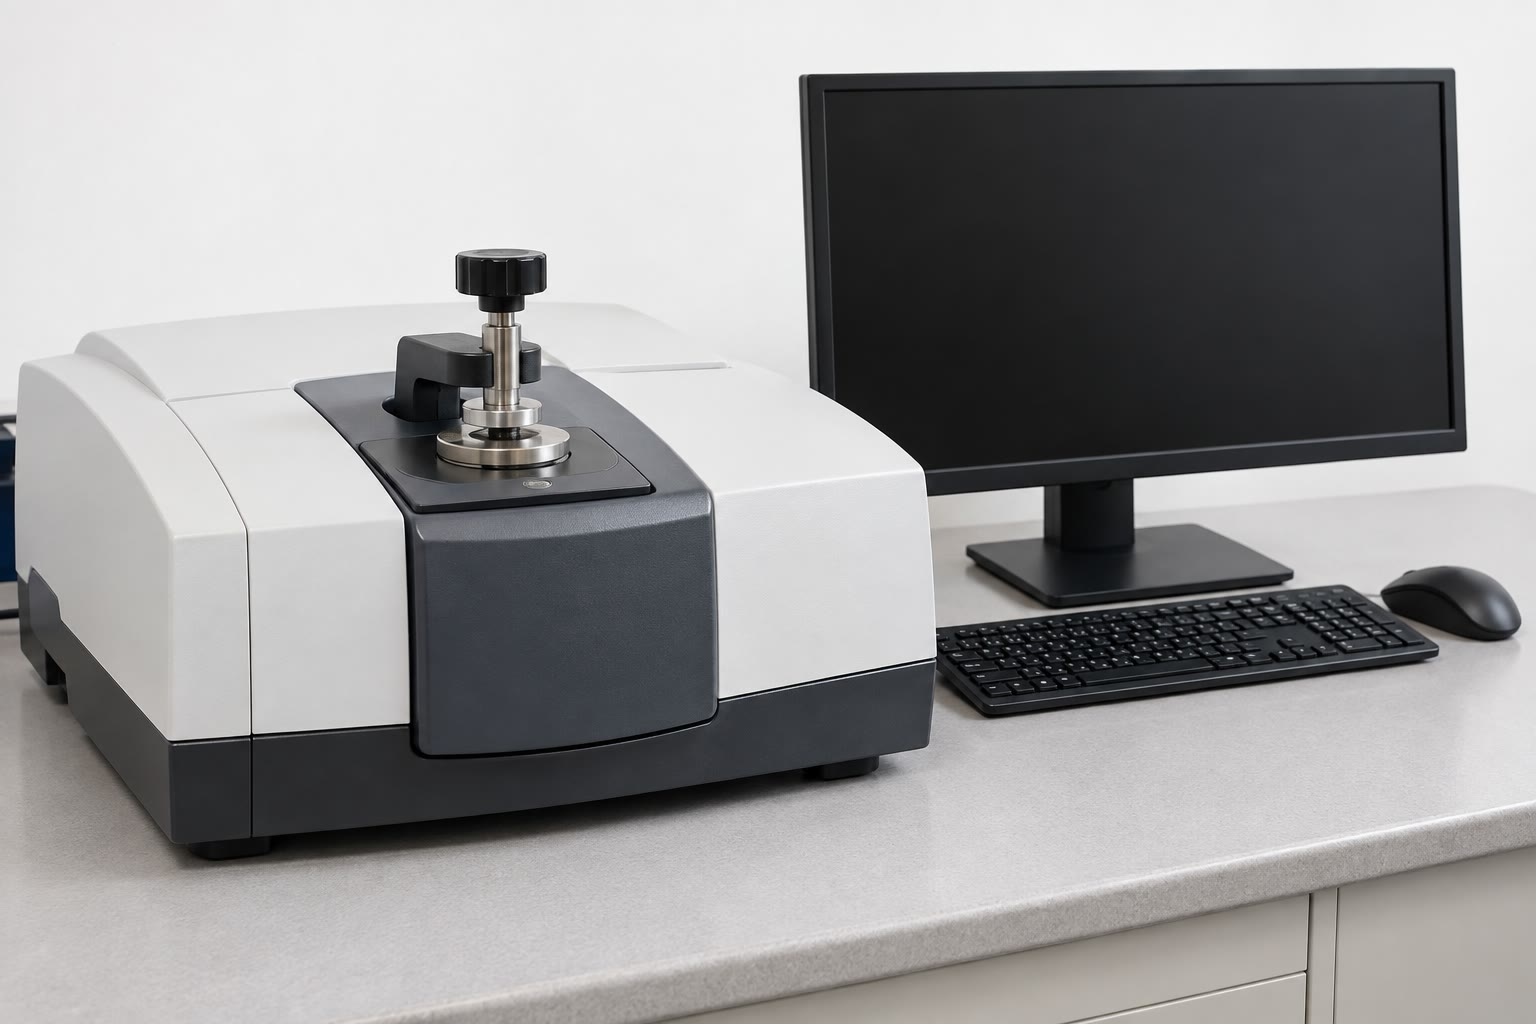
\includegraphics[width=0.48\linewidth]{images/book1/ai/g11-ftir.jpg}

{\small Un espectrómetro infrarrojo de sobremesa con su cristal y su
pinza.}
\end{omfigure}

\begin{omfigure}
\begin{tikzpicture}[font=\small, x=0.0036cm, y=0.5cm]
  % wavenumber axis reversed: x = 4000 - sigma
  \fill[black!8] (2500,0.2) rectangle (3500,7.6);
  \node[font=\footnotesize, align=center, black!60] at (3000,6.8) {huella\\ dactilar};
  \draw[->] (0,0) -- (3600,0) node[right] {$\sigma$};
  \foreach \s in {4000,3500,3000,2500,2000,1500,1000,500}
    \draw ({4000-\s},0) -- ({4000-\s},-0.15) node[below, font=\footnotesize] {\s};
  \node[below=12pt] at (1800,-0.3) {número de onda (\si{cm^{-1}})};
  \foreach \a/\b/\y/\c/\l in {
      3600/3600/7/omDef/{\ce{O-H} libre},
      3300/3400/6/omDef/{\ce{O-H} asociado},
      2500/3300/5/omThm/{\ce{O-H} ácido},
      3300/3500/4/omMeth/{\ce{N-H}},
      2850/2960/3/black!60/{\ce{C-H}},
      1700/1740/2/omProp/{\ce{C=O}},
      1050/1050/1/black!45/{\ce{C-O}}} {
    \fill[\c, rounded corners=1pt] ({4000-\b-12},{\y-0.25}) rectangle ({4000-\a+12},{\y+0.25});
    \node[anchor=west, font=\footnotesize] at ({4000-\a+40},\y) {\l};
  }
\end{tikzpicture}

{\small Dónde absorben los principales enlaces. Las bandas \ce{O-H} y
\ce{N-H} están a la izquierda; la banda \ce{C=O}, por lo general la más
intensa, hacia \qty{1700}{cm^{-1}}; por debajo de \qty{1500}{cm^{-1}}
está la \omterm{def:g11:infrared:band}{región de la huella dactilar}.}
\end{omfigure}

\begin{proposition}[Los enlaces de hidrógeno ensanchan la banda O--H]\label{prop:g11:infrared:hbond}
% ledger: ir:OH-free, ir:OH-bonded, ir:ethanol-OH
Cuando los grupos \ce{O-H} están unidos por \omterm{def:g11:polarity-and-cohesion:hydrogen-bond}{enlaces de hidrógeno}, como
en un \omterm{def:g11:functional-groups:alcohol}{alcohol} líquido, su banda es ancha y está a \omterm{def:g11:infrared:wavenumber}{números de onda} más
bajos (unos 3300--\qty{3400}{cm^{-1}}); sin \omterm{def:g11:polarity-and-cohesion:hydrogen-bond}{enlaces de hidrógeno}, como
en el gas, es estrecha y está hacia \qty{3600}{cm^{-1}}.
\end{proposition}

\begin{proof}
Se admite: un \omterm{def:g11:polarity-and-cohesion:hydrogen-bond}{enlace de hidrógeno} tira del \omterm{def:g7:atoms-and-molecules:atom}{átomo} de hidrógeno y afloja
el enlace \ce{O-H}, que vibra más despacio; y como cada \omterm{def:g7:atoms-and-molecules:molecule}{molécula} está
unida de manera un poco distinta, la banda se extiende en un intervalo.
\end{proof}

\section{Identificar grupos funcionales}


\begin{method}[Leer un espectro infrarrojo]\label{met:g11:infrared:reading}
\begin{enumerate}
  \item Mirar primero por encima de \qty{1500}{cm^{-1}}; dejar la \omterm{def:g11:infrared:band}{región
        de la huella dactilar} para la comparación con espectros
        conocidos.
  \item Hacia \qty{1700}{cm^{-1}}: una banda muy intensa indica un grupo
        \ce{C=O} (\omterm{def:g11:functional-groups:carbonyl}{aldehído}, \omterm{def:g11:functional-groups:carbonyl}{cetona}, ácido, \omterm{def:g11:functional-groups:carboxylic-acid}{éster}, \omterm{def:g11:functional-groups:amine}{amida}).
  \item Entre 2500 y \qty{3700}{cm^{-1}}: una banda ancha hacia
        \qty{3350}{cm^{-1}} indica un \ce{O-H} de \omterm{def:g11:functional-groups:alcohol}{alcohol}; una banda muy
        ancha de 2500 a \qty{3300}{cm^{-1}} junto con un \ce{C=O} indica
        un \omterm{def:g11:functional-groups:carboxylic-acid}{ácido carboxílico}; unas bandas medias a
        3300--\qty{3500}{cm^{-1}} indican \ce{N-H}.
  \item Combinar con la \omterm{def:g11:organic-skeletons:formulas}{fórmula molecular} para elegir la familia, y
        comprobar después con la posición de la banda \ce{C=O}, si la
        hay.
\end{enumerate}
\end{method}

\begin{omfigure}
\newcommand{\irpanel}[2]{%
\begin{tikzpicture}
\begin{axis}[width=0.96\linewidth, height=3.9cm, x dir=reverse, xmin=500,
    xmax=4000, ymin=0, ymax=105, xtick={4000,3000,2000,1000},
    /pgf/number format/1000 sep={},
    ytick={0,50,100}, tick label style={font=\scriptsize},
    label style={font=\scriptsize}, ylabel={$T$ (\%)}, axis lines*=left,
    title={\small #2}, title style={yshift=-4pt}]
  \addplot[thick, omDef] table[x=sigma, y=#1] {figdata/out/grade-11-infrared.dat};
\end{axis}
\end{tikzpicture}}
\begin{minipage}{0.49\linewidth}\irpanel{ethanolL}{A: etanol (líquido)}\end{minipage}\hfill
\begin{minipage}{0.49\linewidth}\irpanel{ethanolG}{B: etanol (gas)}\end{minipage}

\begin{minipage}{0.49\linewidth}\irpanel{propanone}{C: propanona}\end{minipage}\hfill
\begin{minipage}{0.49\linewidth}\irpanel{acid}{D: ácido etanoico}\end{minipage}

\begin{minipage}{0.49\linewidth}\irpanel{ester}{E: etanoato de etilo}\end{minipage}\hfill
\begin{minipage}{0.49\linewidth}\irpanel{amine}{F: etanamina}\end{minipage}

{\small \omterm{def:g11:infrared:spectrum}{Espectros infrarrojos} de seis compuestos, con el \omterm{def:g11:infrared:wavenumber}{número de onda}
en \si{cm^{-1}} (decreciente hacia la derecha). Solo se dibujan las
bandas que se comentan en el capítulo; sus posiciones proceden de
espectros medidos y de tablas, y su forma, de un modelo sencillo.}
\end{omfigure}

\begin{example}[Leer los seis espectros]\label{ex:g11:infrared:six}
% ledger: ir:OH-bonded, ir:ethanol-OH, ir:CO-ketone, ir:OH-acid, ir:CO-acid, ir:CO-ester, ir:ethylethanoate-COC, ir:NH
El etanol (A) presenta una banda \ce{O-H} ancha hacia
\qty{3350}{cm^{-1}}, las bandas \ce{C-H} justo por debajo de
\qty{3000}{cm^{-1}} y una banda \ce{C-O} intensa hacia
\qty{1050}{cm^{-1}}, pero nada hacia \qty{1700}{cm^{-1}}. En el gas (B),
su banda \ce{O-H} se convierte en una línea estrecha a
\qty{3666}{cm^{-1}}. La propanona (C) no tiene banda \ce{O-H}, pero sí
un \ce{C=O} muy intenso a \qty{1715}{cm^{-1}}. El ácido etanoico (D)
presenta las dos cosas: una enorme banda \ce{O-H} de 2500 a
\qty{3300}{cm^{-1}} y un \ce{C=O} a \qty{1710}{cm^{-1}}. El etanoato de
etilo (E) tiene su \ce{C=O} a \qty{1735}{cm^{-1}} y un \ce{C-O} intenso
hacia \qty{1240}{cm^{-1}}, y ningún \ce{O-H}. La etanamina (F) presenta
dos bandas \ce{N-H} medias por encima de \qty{3300}{cm^{-1}}.
\end{example}

\section{Ejercicios}

\begin{exercise}[$\star$]\label{exo:g11:infrared:1}
Convierte en una longitud de onda en micrómetros:
$\sigma = \qty{3300}{cm^{-1}}$ y $\sigma = \qty{1050}{cm^{-1}}$. ¿Cuál
corresponde a la vibración más rápida?
\end{exercise}

\begin{exercise}[$\star$]\label{exo:g11:infrared:2}
Se absorbe una longitud de onda de \qty{10}{\micro m}. Da el \omterm{def:g11:infrared:wavenumber}{número de
onda} en \si{cm^{-1}}.
\end{exercise}

\begin{exercise}[$\star$]\label{exo:g11:infrared:3}
¿Qué enlace absorbe: hacia \qty{1715}{cm^{-1}}; hacia
\qty{3350}{cm^{-1}} (banda ancha); entre 2850 y \qty{2960}{cm^{-1}}?
\end{exercise}

\begin{exercise}[$\star$]\label{exo:g11:infrared:4}
En el espectro C (propanona), busca la banda más intensa. ¿A qué enlace
pertenece?
\end{exercise}

\begin{exercise}[$\star$]\label{exo:g11:infrared:5}
¿Por qué un \omterm{def:g11:infrared:spectrum}{espectro infrarrojo} se dibuja con un eje de \omterm{def:g11:infrared:spectrum}{transmitancia},
con las bandas hacia abajo? ¿Qué significa $T = \qty{100}{\percent}$?
\end{exercise}

\begin{exercise}[$\star\star$]\label{exo:g11:infrared:6}
Un compuesto \ce{C4H8O} presenta una banda muy intensa a
\qty{1715}{cm^{-1}} y ninguna banda por encima de \qty{3000}{cm^{-1}}.
Otro, \ce{C4H10O}, presenta una banda ancha hacia \qty{3350}{cm^{-1}} y
ninguna hacia \qty{1700}{cm^{-1}}. ¿A qué familias pertenecen? Propón un
nombre para cada uno.
\end{exercise}

\begin{exercise}[$\star\star$]\label{exo:g11:infrared:7}
Explica por qué la banda \ce{O-H} del ácido etanoico es tan ancha, más
ancha incluso que la del etanol líquido.
\end{exercise}

\begin{exercise}[$\star\star$]\label{exo:g11:infrared:8}
Compara los espectros A y B del etanol. ¿Qué cambia, y por qué?
\end{exercise}

\begin{exercise}[$\star\star$]\label{exo:g11:infrared:9}
El propanal y la propanona son los dos \ce{C3H6O}. Los dos presentan una
banda \ce{C=O} intensa. ¿Puede el infrarrojo distinguirlos solo con esa
banda? ¿Qué más podría ayudar?
\end{exercise}

\begin{exercise}[$\star\star$]\label{exo:g11:infrared:10}
Un compuesto presenta una banda intensa a \qty{1735}{cm^{-1}}, una banda
intensa hacia \qty{1240}{cm^{-1}} y nada por encima de
\qty{3000}{cm^{-1}}. Su fórmula es \ce{C4H8O2}. ¿Qué familia? ¿Es
posible el ácido etanoico? ¿Y el ácido butanoico?
\end{exercise}

\begin{exercise}[$\star\star$]\label{exo:g11:infrared:11}
¿A cuál de los seis espectros se parecería más una \omterm{def:g7:atoms-and-molecules:molecule}{molécula} de
propan-1-ol? ¿Y una de ácido propanoico? Explícalo.
\end{exercise}

\begin{exercise}[$\star\star\star$]\label{exo:g11:infrared:12}
El propan-2-ol se puede oxidar a propanona. Una alumna sigue la reacción
registrando los espectros de muestras tomadas cada diez minutos.
Describe cómo cambian los espectros. ¿Cómo sabe que la reacción ha
terminado?
\end{exercise}

\begin{exercise}[$\star\star\star$]\label{exo:g11:infrared:13}
El ácido butanoico y el etanoato de etilo son \omterm{def:g11:organic-skeletons:isomer}{isómeros}, \ce{C4H8O2}.
Describe dos diferencias entre sus \omterm{def:g11:infrared:spectrum}{espectros infrarrojos}, y explícalas.
\end{exercise}

\begin{exercise}[$\star\star\star$]\label{exo:g11:infrared:14}
Una muestra de etanoato de etilo presenta, además de las bandas
esperadas, una banda débil y ancha hacia \qty{3350}{cm^{-1}}. Propón dos
impurezas que podrían causarla (piensa en cómo se fabrican los \omterm{def:g11:functional-groups:carboxylic-acid}{ésteres},
y en el \omterm{def:g4:air-a-mixture-of-gases:air}{aire}). ¿Cómo se podría comprobar la muestra?
\end{exercise}

\begin{exercise}[$\star\star\star$]\label{exo:g11:infrared:15}
La banda \ce{C=O} de las \omterm{def:g11:functional-groups:carbonyl}{cetonas} está hacia \qty{1715}{cm^{-1}}, la de
un \ce{C=C} hacia \qty{1650}{cm^{-1}}, y la banda \ce{C-O} hacia
\qty{1050}{cm^{-1}}. Con la imagen de las dos bolas unidas por un muelle,
explica por qué un \omterm{def:g10:lewis-and-shape:multiple-bond}{enlace doble} \ce{C=O} vibra más deprisa que un enlace
sencillo \ce{C-O}. ¿Por qué las bandas \ce{O-H}, \ce{N-H} y \ce{C-H}
están todas a \omterm{def:g11:infrared:wavenumber}{números de onda} altos?
\end{exercise}

\section{Problema: Tres frascos sin etiqueta}

\begin{problem}[{Problema de fin de semana --- tres frascos han perdido
sus etiquetas: ¿cuál es cuál, y qué longitud de onda absorbe más la
cetona?}]
\label{pb:g11:infrared:1}
% ledger: ir:OH-bonded, ir:OH-acid, ir:CO-ketone, ir:CO-acid, ir:CO-single
Tres frascos de líquido incoloro han perdido sus etiquetas. La lista
del almacén dice que contienen etanol, propanona y ácido etanoico. Se
registran sus espectros: el frasco 1 da un espectro como el A; el
frasco 2, como el D; y el frasco 3, como el C.

\medskip
\noindent\textbf{Parte I --- Los candidatos.}
\begin{enumerate}
  \item Escribe las \omterm{def:g11:organic-skeletons:formulas}{fórmulas semidesarrolladas} del etanol, la propanona
        y el ácido etanoico.
  \item Da sus \omterm{def:g11:organic-skeletons:formulas}{fórmulas moleculares}.
  \item Nombra el \omterm{def:g11:functional-groups:functional-group}{grupo funcional} de cada uno.
  \item ¿Qué enlaces de cada uno deberían dar una banda por encima de
        \qty{1500}{cm^{-1}}?
\end{enumerate}

\medskip
\noindent\textbf{Parte II --- Los espectros.}
\begin{enumerate}[resume]
  \item Frasco 1: ¿hay una banda \ce{C=O}? ¿Una banda \ce{O-H}? ¿Qué
        compuesto es?
  \item Frasco 2: describe sus dos rasgos más marcados. ¿Qué compuesto?
  \item Frasco 3: ¿qué compuesto? ¿Qué banda lo decide?
  \item ¿Habría podido distinguirlos el olor? ¿Por qué es mejor no
        intentarlo?
  \item ¿Por qué la banda \ce{O-H} del frasco 2 es más ancha que la del
        frasco 1?
\end{enumerate}

\medskip
\noindent\textbf{Parte III --- \omterm{def:g11:organic-skeletons:isomer}{Isómeros}.}
\begin{enumerate}[resume]
  \item El metoximetano es un \omterm{def:g11:organic-skeletons:isomer}{isómero} del etanol. Escribe su fórmula.
        ¿Qué banda del etanol le faltaría a su espectro?
  \item El propanal es un \omterm{def:g11:organic-skeletons:isomer}{isómero} de la propanona. ¿Qué banda comparten?
        ¿Dónde está en cada uno?
  \item El metanoato de metilo, \ce{HCOO-CH3}, es un \omterm{def:g11:organic-skeletons:isomer}{isómero} del ácido
        etanoico. ¿Qué banda del ácido faltaría? ¿Dónde estaría su banda
        \ce{C=O}?
  \item ¿Por qué una \omterm{def:g11:organic-skeletons:formulas}{fórmula molecular} sola no permite identificar un
        compuesto, mientras que la fórmula y el espectro juntos suelen
        permitirlo?
\end{enumerate}

\medskip
\noindent\textbf{Parte IV --- La longitud de onda.}
\begin{enumerate}[resume]
  \item ¿Cuál es el \omterm{def:g11:infrared:wavenumber}{número de onda} de la banda más intensa de la
        propanona?
  \item Exprésalo en \si{m^{-1}}.
  \item Calcula la longitud de onda absorbida, en metros y después en
        micrómetros.
  \item ¿Es visible esa luz? ¿A qué tipo de radiación pertenece?
  \item Haz lo mismo con la banda \ce{C-O} del etanol hacia
        \qty{1050}{cm^{-1}}.
  \item ¿Cuál de los dos enlaces vibra más deprisa?
  \item Da la respuesta final: ¿qué longitud de onda absorbe con más
        intensidad el enlace \ce{C=O} de la propanona?
\end{enumerate}
\end{problem}
